\begin{frame}{Cloud}
    Essentially, it is a term used to describe a global network of servers, which are hooked together and meant to operate as a single ecosystem.
    \begin{center}
        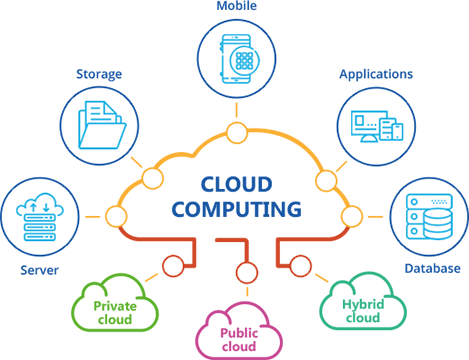
\includegraphics[width=0.5\textwidth]{img/cloud-computing.png}
    \end{center}
\end{frame}

\begin{frame}{Cloud Services}
    \begin{center}
        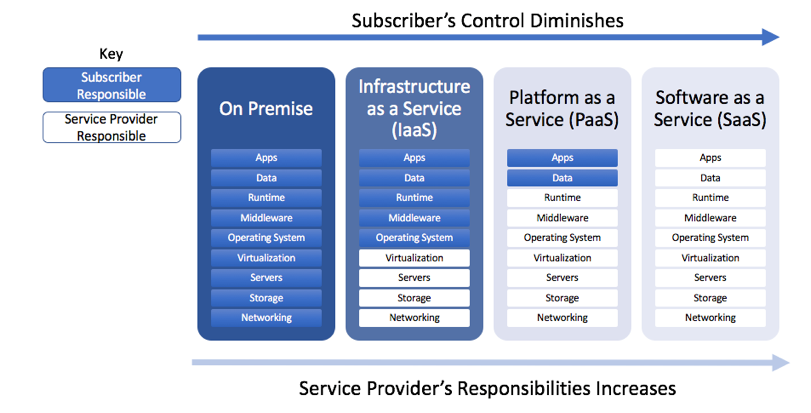
\includegraphics{img/cloud-services-model.png}
    \end{center}
\end{frame}

\begin{frame}{Pros \& Cons}
    \begin{block}{Pros}
        \begin{itemize}
            \item Reduced hardware equipment for end-users
            \item Improved performance
            \item Lower H/W and S/W maintainence
            \item Instant software updates
            \item Improved disaster recovery
            \item Less expensive
            \item Accessibility
        \end{itemize}
    \end{block}

    \begin{block}{Cons}
        \begin{itemize}
            \item Requires good internet connection \& bandwidth
            \item Limited control on infrastructure
        \end{itemize}
    \end{block}
\end{frame}

\begin{frame}{Problem Statement}
    \begin{block}{Experimental Cloud using Commodity Hardware}
        The objective of this project is to create an experimental cloud by repurposing commodity hardware. The cloud we create would be made available to students as virtual desktops which may be used to host web services which can vary from simple static page to complex web applications.
    \end{block}
\end{frame}